AGREE translates an AADL model and its annotated contracts into a dialect \cite{jkind} of the Lustre language, and then queries a user-selected model checker to perform the verification. The dialect includes an expression called \emph{condact}, which is similar to the activation condition in SCADE. It clocks a node call expression as follows: 
$
condact (cond, node(node\_inputs, node\_outputs), init\_outputs)
$.
If the Boolean signal $cond$ is true, the clocked node $node$ is activated and updates its local and output signals. Otherwise, the node keeps the previous value of the local and output signals. Before the first activation, the node outputs values are set to \emph{init\_outputs}.
We are aware that the standard Lustre language introduced similar temporal operators like \emph{when} and \emph{current}. We use \emph{condact} simply because it is supported by our default model checker JKind \cite{jkind}.

AGREE translates an AADL thread to a Lustre node in a \emph{constraint} style, in which the thread input and output ports are both mapped to the node input signals. Thus, the \emph{condact} expression does not automatically freeze the thread outputs. We add assertions to enforce the output freeze rule, and we use the thread \emph{complete} signal to clock the node. The \emph{complete} signal is triggered by the circular counter shown in Figure~\ref{schedule}. Figure~\ref{WPMlustre} shows an example of using \emph{condact} to model a scheduled AADL thread. 

\begin{figure}[t!]
\centering
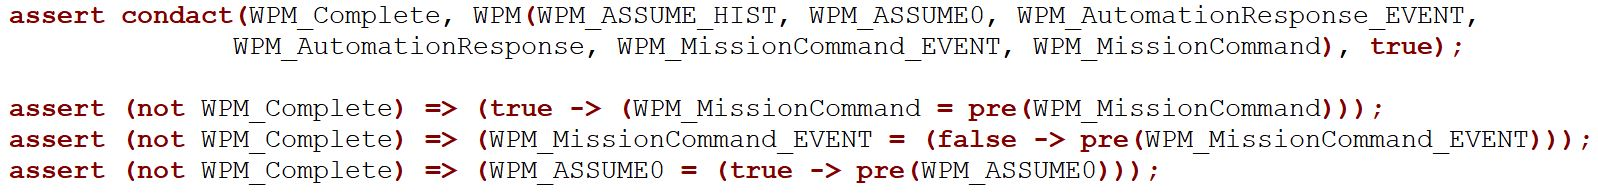
\includegraphics[width=120mm]{lustreAsync5.jpg}
\caption{Modeling Scheduling Semantics with \emph{condact} in Lustre \label{WPMlustre}}
\end{figure}
  
